\newpage
\section{Notations}
\label{sec:appendix-notations}

For completeness, we provide a list of notations we used in the paper, reported in Table \ref{tab:notations}.
% We also list the parameters of the main components in GQA Transformers and their corresponding FLOPs in Table~\ref{tab:costs-components}.

\begin{table}[!t]
    \centering
    \footnotesize
    \begin{tabular}{l|p{5.6cm}}
        \toprule
        \textbf{Notation} & \textbf{Meaning} \\
        \bottomrule
        \toprule  
        \multicolumn{2}{c}{\textit{Model hyperparameters}}\\
        \midrule
        $V$ & Vocabulary size, always set to 50,304. \\
        \midrule
        $L$ & Number of layers \\
        \midrule
        $d$ & Model hidden dimension \\
        \midrule
        $d_h$ & Head size, always set to $64$. \\
        \midrule
        $d_\text{ff}$ & FFN intermediate size, we always set $d_\text{ff}=8d/3$. \\
        \midrule
        $\sigma$ & The activation function in FFN \\
        \midrule
        $n_h$ & Number of attention heads \\
        \midrule
        $n_{kv}$ & Number of KV heads (or groups in GQA) \\
        \bottomrule
        \toprule
        \multicolumn{2}{c}{\textit{Inference and Training Costs}}\\
        \midrule
        $C_\text{infer}$ & The computational cost (in FLOPs) per forward pass with a context length of $T$ tokens.\\
        \midrule
        $M_\text{infer}$ & The memory usage (in floating-point values) of serving the model with a context length of $T$ tokens. \\
        \midrule
        $C_\text{train}$ & The computational cost (in FLOPs) used to train the model with a context length of $T$ tokens.\\
        \midrule
        $M_\text{train}$ & The memory usage (in floating-point values) of training the model with a context length of $T$ tokens. \\
        \midrule
        $Z$   & Hardware-aware costs combining both $M_\text{infer}$ and $C_\text{infer}$. Defined in Section~\ref{sec:cost-optimal-gqa-search}.\\
        \bottomrule
        \toprule
        \multicolumn{2}{c}{\textit{Other parameters}}\\
        \midrule
        $T$ & Context length \\
        \midrule
        $N$ & Number of model parameters. \\
        \midrule
        $D_\text{train}$ & Number of training tokens. \\
        \midrule
        $\lambda,\alpha,\beta$ & Hyperparameters controlling the importance of memory and compute resources.\\
        \bottomrule
    \end{tabular}
    \caption{List of notations used in the paper.}
    \label{tab:notations}
\end{table}

\section{Discussions}

% \paragraph{Do the Compute and Memory Usage Reflect Actual Throughput?}

% In practice, FLOPs and memory usage may not reflect actual throughput. However, throughput is highly dependent on the downstream hardware, so if the goal is to optimize the loss and throughput tradeoffs, we should measure the actual speed and try to model loss as a function of speed. This has two problems. (1) The conclusions are not generalizable to new hardware, and since new hardware is constantly being developed, minimizing FLOPs and memory usage may be more beneficial in the long term. (2) There is no simple formula for throughput, which makes it hard to model the relationship between loss and throughput. Due to these two problems, we have focused on minimizing FLOPs and memory usage.

\paragraph{What About Other Efficient Attention?}

This paper primarily adjusts the allocation of compute and memory usage by tweaking the model size (controlled with $L$ and $d$) and head configuration $(n_h, n_{kv})$ in GQA, which is a rather simple method. As mentioned, there are many techniques for improving the efficiency of the attention layer, although those have enjoyed less adoption. When using these techniques, the computational and memory costs may be considerably different, and some of our conclusions may not apply. Despite so, our work is still a valuable improvement over existing implementations of GQA.

Recently, Multi-head Latent Attention (MLA) \citep{deepseek-v2} was proposed as a strong alternative to GQA for reducing the KV cache size. During inference, MLA reformulates the attention computation such that all heads share a unified representation for keys and values. In this case, our analysis still applies, since MLA can be seen as a kind of GQA with a different head dimension ($d_h$) and number of attention heads ($n_h, n_{kv}$), and it uses a more complex function to generate the QKV vectors.

\paragraph{What If Context Length Varies?}

The formulas for computational costs (see Table~\ref{tab:costs-full}) are affine functions of $T$, so the \textit{expected costs} are:
\begin{align*}
\mathbb E(C_\text{infer}(T)) &= C_\text{infer}(\mathbb E(T)) \\
\mathbb E(M_\text{infer}(T)) &= M_\text{infer}(\mathbb E(T)) \\
\mathbb E (C_\text{train}(T_\text{train})) &= C_\text{train}(\mathbb E(T_\text{train}))\\
\mathbb E(M_\text{train}(T_\text{train})) &= M_\text{train}(\mathbb E(T_\text{train}))
\end{align*}
where $T_\text{train}$ is the context length during training.
Hence, it suffices to compare the costs with the expected context length. 

\paragraph{Will the Findings Break Down When Scaling Up the Model/Data Size?}

This is a never-ending argument against most neural architectural changes, because no matter the scale of our experiments, we can never be sure that the behavior holds for larger scales. However, our experiments have already covered model sizes up to 1.2B, which is already the size of some widely-used models at the moment \citep{llama3,qwen2.5}. Empirically, it has been widely validated that the scaling law is highly predictable to a good extent beyond the largest model (e.g., Llama-3 accurately predicted the loss of a 405B model with experiments on model sizes up to 16B). Thus, we are confident that our conclusions hold at least for models up to 10B parameters.

\subsection{How to Calculate the Costs of Models of Arbitrary Sizes?} 
\label{sec:appendix-cost-of-arbitrary-size}

\begin{table}[!t]
    \centering
    \begin{tabular}{c|ccc}
        \toprule
        $N$ & $L$ & $d$ \\
        \midrule
        1.2B & 36 & 1536 \\
        1.8B & 36 & 2048 \\
        4B  & 48 & 2560 \\
        6B  & 54 & 3072 \\
        13B & 64 & 4096 \\
        33B & 72 & 6144 \\ 
        64B & 80 & 8192 \\
        \bottomrule
    \end{tabular}
    \caption{The pre-defined configurations used to calculate the aspect ratio of arbitrarily sized models. For models smaller than 1.2B, we use the configurations in Table~\ref{tab:vanilla-model-configs}.}
    \label{tab:aspect-ratio-configs}
\end{table}

In step 3 of our procedure (proposed in Section~\ref{sec:cost-optimal-gqa-search}), we arrive at a critical model size $N^*(H)$. It is a real value, so it does not correspond to an actual model configuration. To calculate the inference costs $(M_\text{infer}, C_\text{infer}, Z)$ of a model of this size, we need $H$ and the aspect ratio of the model $a=d/L$. $H$ is already given, which may be a function of $d$. For the aspect ratio, we perform linear interpolation between the nearest two pre-defined model configurations. The pre-defined model aspect ratios are given in Table~\ref{tab:aspect-ratio-configs}. Then, we use binary search to find the $L$ that corresponds to $N^*(H)$. We can calculate $d$ from $L$ and $a$. Then, we calculate $n_h$ and $n_{kv}$ from $d$ and the specified configuration. With all these values (non-integers) known, we can calculate the model size as well as the inference costs.

To produce an actual model in practice, we suggest simply choosing the configuration $(N,n_h,n_{kv})$ closest to the derived answer in step 3. The slight variations in the performance of the resulting configuration are negligible compared to the huge cost savings gained by selecting the cost-optimal configuration using our approach.


\section{Training Costs of GQA Transformers}
\label{sec:appendix-training-costs}

\begin{table}[t]
    \centering
    \small
    \begin{tabular}{l|cc}
        \toprule
            \textbf{Cost Type}
            & \textbf{Time-invar.} 
            & \textbf{Time-var.}\\
        \midrule
        Infer. FLOPs $(C_\text{infer})$
            & $2N$ 
            & $4TLd_hn_{h}$  \\
        Infer. Mem. $(M_\text{infer})$ 
            & $N$ 
            & $2TLd_hn_{kv}$ \\
        \midrule
        Train. FLOPs $(C_\text{train})$  
            & $6D_\text{train}N$ 
            & $12D_\text{train}TLd_hn_{h}$ \\
        Train. Mem. $(M_\text{train})$
            & $4N$ 
            & $TdL$ \\
        \bottomrule
    \end{tabular}
    \caption{The time-invariant and time-variant costs of GQA Transformers during inference and training.}
    \label{tab:costs-full}
\end{table}


\paragraph{Training Computational Costs}

In addition to inference costs, different head configurations also result in different training costs, because the number of training FLOPs, $C_\text{train}$, is a function of $C_{\text{infer}}$.
Following \citet{scaling-law}, we estimate the FLOPs of the backward pass as double the FLOPs of the forward pass. Let $D_\text{train}$ denote the number of training tokens, $T_i$ denotes the number of tokens preceding the $i$-th training token in the training corpora, then the training FLOPs are:
\begin{align}
C_\text{train} 
    &\approx 3D_\text{train}C_{\text{infer}} \left(\overline T \right) \\
    &= 6D_\text{train} ( 
        N + \underbrace{2L \overline T d_h n_h}_\text{Attention}
    ),
    \label{eq:training-compute}
\end{align}
where $\overline T$ is the average value of $\{T_i|i=1, \cdots, D_\text{train}\}$. When all examples in the training corpora are set to the constant length $T_\text{train}$, during training, we have $\overline T = T_\text{train}/2$. However, in practice, when training long-context LLMs, it is more common to use short contexts for most of the time, and only use long contexts consisting of a small number of tokens to adapt the model to the target context length. Hence, the time-variant FLOPs may only make up a small portion of the training FLOPs, making the cost largely independent of the GQA configuration. Consequently, our paper considers training costs, but focuses more on optimizing inference costs.

\paragraph{Training Memory Costs} 

We only need to store model parameters, activations, gradients, and optimizer states during training. Assuming the widely-used Adam \citep{adam} optimizer without offloading any storage to the CPU, the memory cost is roughly:
% \footnote{When using FlashAttention \citep{flash-attention-2} to avoid storing attention scores, attention blocks only require a constant memory cost.}
\begin{align}
M_\text{train}(T) \approx 4N + \underbrace{TdL}_\text{Activations}.
\end{align}
While it is important to lower the cost of caching activations when $T$ is large, we do not have a free hyperparameter to adjust this cost (like $n_h$ for computational costs and $n_{kv}$ for memory costs). To reduce the size of activations, we have to modify $d$ and/or $L$, which either drastically changes the model size or its aspect ratio. Either of such changes leads to major consequences that are beyond the scope of this paper. Regarding the $4N$ part of training memory cost, it is only dependent on the total model size, so it suffices to minimize the model size, which is already addressed in many existing works \citep{scaling-law,llama3,beyond-chinchilla}.

% \begin{figure*}[t]
%     \centering
%     \includegraphics[width=1.0\linewidth]{figures/loss-by-costs/fig1.pdf}
%     \caption{The main results. It shows LM loss as a function of memory and computational costs during inference when the context length is 128K tokens, assuming we use BF16 for both model parameters and KV cache. $H=(n_h,n_{kv})$ denotes the number of attention heads and KV heads. The x-axis is on the log scale. The result shows that the widely used GQA configuration ($H=(d/d_h, 8)$) is suboptimal.}
%     \label{fig:loss-vs-flops}
% \end{figure*}










\begin{figure*}[!t]
    \centering
    \begin{minipage}{0.32\textwidth}
        \centering
        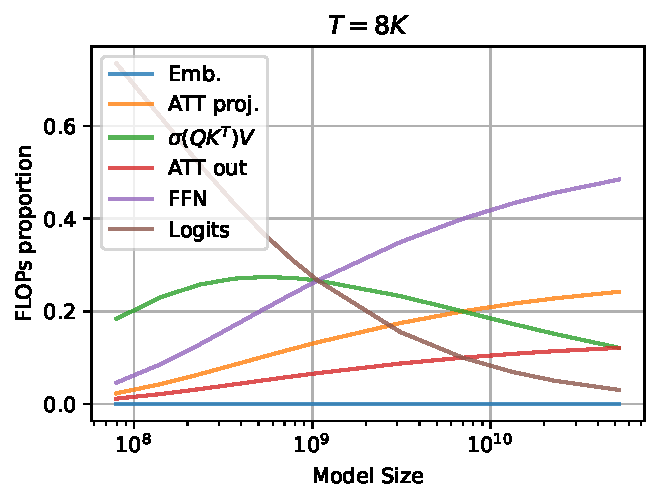
\includegraphics[width=\textwidth]{figures/costs-by-model-size/flops_by_model_size_8k.pdf}
        % \subcaption{T=8K}
        \label{fig:flops_distr_subfig1}
    \end{minipage}
    \hfill
    \begin{minipage}{0.32\textwidth}
        \centering
        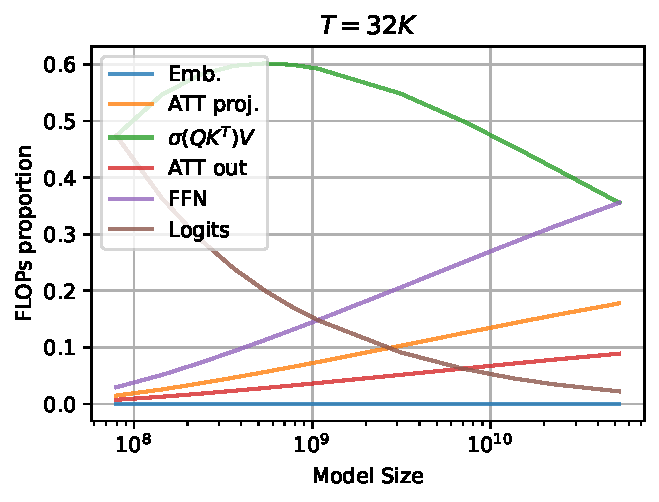
\includegraphics[width=\textwidth]{figures/costs-by-model-size/flops_by_model_size_32k.pdf}
        % \subcaption{Subfigure 2}
        \label{fig:flops_distr_subfig2}
    \end{minipage}
    \hfill
    \begin{minipage}{0.32\textwidth}
        \centering
        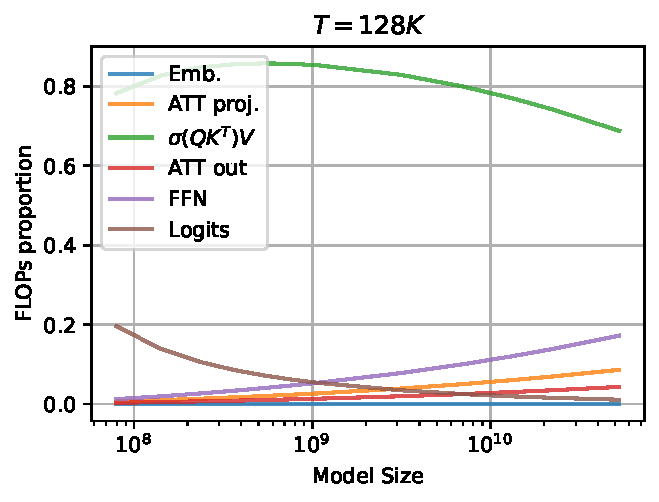
\includegraphics[width=\textwidth]{figures/costs-by-model-size/flops_by_model_size_128k.pdf}
        % \subcaption{Subfigure 3}
        \label{fig:flops_distr_subfig3}
    \end{minipage}
    \caption{The proportion of FLOPs allocated to different components in a Transformer LM, with multi-head attention and RoPE. As the context length increases, most FLOPs are spent on the time-variant computation of the attention operator $\sigma(\mathbf Q\mathbf K^\top)\mathbf V$, where $\sigma$ is the row-wise softmax function.}
    \label{fig:flops_distr_by_model_size}
\end{figure*}


\begin{figure*}[!t]
    \centering
    \begin{minipage}{0.32\textwidth}
        \centering
        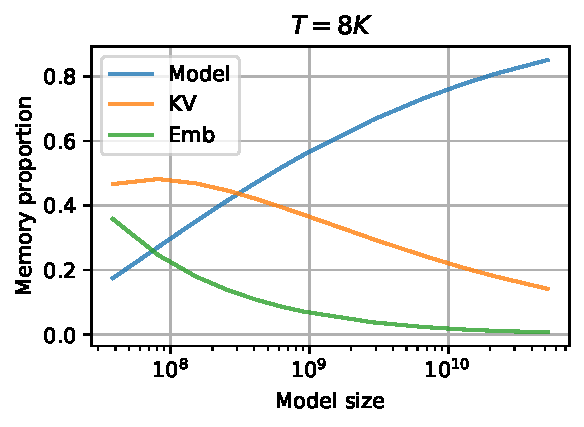
\includegraphics[width=\textwidth]{figures/costs-by-model-size/mem_by_model_size_8k.pdf}
        % \subcaption{T=8K}
        \label{fig:mem_subfig1}
    \end{minipage}
    \hfill
    \begin{minipage}{0.32\textwidth}
        \centering
        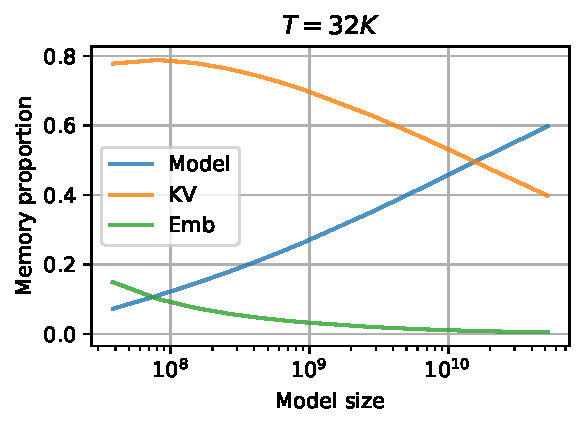
\includegraphics[width=\textwidth]{figures/costs-by-model-size/mem_by_model_size_32k.pdf}
        % \subcaption{Subfigure 2}
        \label{fig:mem_subfig2}
    \end{minipage}
    \hfill
    \begin{minipage}{0.32\textwidth}
        \centering
        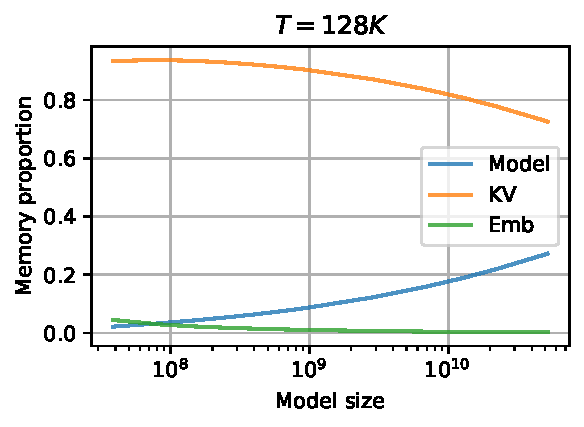
\includegraphics[width=\textwidth]{figures/costs-by-model-size/mem_by_model_size_128k.pdf}
        % \subcaption{Subfigure 3}
        \label{fig:mem_subfig3}
    \end{minipage}
    \caption{The proportion of memory allocated to different components in a Transformer LM, with multi-head attention and RoPE. As the context lengths increase, most of the memory usage is spent on storing the KV cache.}
    \label{fig:mem_distr_by_model_size}
\end{figure*}












\section{Model Configurations}
\label{sec:appendix-model-config}

Table~\ref{tab:vanilla-model-configs} shows the configurations of the models in our experiments for fitting the scaling law. In general, we ensure that $d_h=64$, $d_\text{ff} \approx 8d/3$ (rounded to the closest multiple of 32) when scaling the model size, which is adopted from common hyperparameters found in existing LLMs such as GPT \citep{gpt} and Llama \citep{llama3}. We also ensure that the aspect ratio $d/L$ is similar to those used by existing modeling scaling works \citep{pythia,chinchilla,qwen2.5}.
We use the GPT-2 tokenizer, which has a vocabulary size of 50,304, and we tie the input and output embeddings. 

\paragraph{Learning Rate}

The maximum learning rate (LR) is chosen by a grid search on $\{1\times10^i,2\times 10^i,5\times 10^i\mid i=-3, -4, -5\}$ with the vanilla MHA, and choosing the one with best LM loss. Then, we just keep the LR the same across different GQA configurations. While different configurations may have different optimal LR, exhaustively sweeping all LR for each configuration is prohibitively expensive.

\paragraph{Differences From Vanilla GPT}

Compared to the vanilla GPT model \citep{gpt}, we make the following changes to better align with more recent LLMs:
\begin{itemize}
    \item We use RoPE \citep{rope} with a $\theta$ value of 500,000, which is widely used in current LMs \citep{llama3}.
    \item We use SwiGLU FFN instead of the ReLU FFN in GPT.
    % \item The model uses ordinary FFNs (one up projection followed by one down projection) instead of gated FFNs to keep the model architecture as simple as possible. Our preliminary experiments found that using gated activation units in FFNs resulted in very small change in language modeling loss. Moreover, we also use SILU activation function instead of GELU in the original GPT model \citep{gelu}.
    \item We use pre-norm \citep{pre-ln} and use RMSNorm \citep{rmsnorm} instead of LayerNorm \citep{layernorm}, which is more common in current LLMs. The epsilon in RMSNorm is $10^{-6}$.
    \item Our model has no bias terms or dropout, which is also common practice and can slightly increase the training efficiency.
\end{itemize}

\begin{table}[!t]
    \centering
    \begin{tabular}{c|ccccc}
        \toprule
        Model size & $L$ & $d$ & $d_h$ & LR \\
        \midrule
        % 197K & 1  & 128   & 2  & 64 & 512 \\
        % 1.6M & 2  & 256   & 4  & 64 & 1,024 \\
        % 13M  & 4  & 512   & 8  & 64 & 2,048 \\
        % 42M  & 6  & 768   & 12 & 64 & 3,072 \\
        % 100M & 8  & 1,024 & 16 & 64 & 4,096 \\
        % 197M & 10 & 1,280 & 20 & 64 & 5,120 \\
        % 340M & 12 & 1,536 & 24 & 64 & 6,144 \\
        % 540M & 14 & 1,792 & 28 & 64 & 7,168 \\
        % 805M & 16 & 2,048 & 32 & 64 & 8,192 \\

        3M   & 4  & 256  & 64 & 1e-3 \\
        19M  & 6  & 512  & 64 & 1e-3 \\
        85M  & 12 & 768  & 64 & 1e-3 \\
        150M & 12 & 1024 & 64 & 1e-3 \\
        200M & 16 & 1024 & 64 & 5e-4 \\
        470M & 24 & 1280 & 64 & 5e-4 \\
        680M & 24 & 1536 & 64 & 2e-4 \\
        1.2B & 36 & 1536 & 64 & 2e-4 \\
        \bottomrule
    \end{tabular}
    \caption{The configurations of the vanilla models with MHA in our experiments, we try to keep it as close to the configurations from \citet{pythia} as possible.}
    \label{tab:vanilla-model-configs}
\end{table}


\section{Data Processing}
\label{sec:appendix-data-processing}

In most of our experiments, we used SlimPajama \citep{slimpj}. We append an EOS token to each document in the corpus before chunking the documents into the specified training length. If the last chunk is shorter than the specified training length, it will be discarded.


\section{Training Configurations}
\label{sec:appendix-training-config}

Here, we provide the default training configurations we used during the experiments.

\begin{itemize}
    \item \textbf{Optimizer:} We use the widely-used AdamW optimizer \citep{adam}, with $\beta_1 =0.9, \beta_2=0.95$, and a weight decay of 0.1. We only apply weight decay to linear layers, which excludes the re-scaling factor in RMSNorm. We also use a gradient clipping value of 1.0.
    \item \textbf{Learning rate scheduler:} We use the warmup-stable-decay (WSD) LR scheduler \citep{minicpm}, with a maximum LR of $5\cdot 10^{-4}$, 10\% warmup steps steps and 20\% decay steps. Warmup starts from 0 and increases linearly to the maximum LR. The decay stage uses a cosine annealing scheme, where the minimum LR is 10\% of the maximum LR.
    \item \textbf{Batch size:} 512K tokens.
    \item \textbf{Floating-point precision:} We use BF16 during training and FP16 during evaluation.
\end{itemize}

\paragraph{Hardware}

All training experiments were run on A800 GPUs, mostly with 8 GPUs.

\section{Memory and Compute Allocations by Model Size}
\label{sec:appendix-memory-and-flops-allocations}

Figure \ref{fig:flops_distr_by_model_size} and \ref{fig:mem_distr_by_model_size} show the FLOPs and memory breakdown of different components as a function of model size. One can see that changes in the model size and/or context length can influence the allocation of FLOPs and memory between different components in the model. For instance, when the context has 128K tokens, the vast majority of FLOPs is spent computing the attention scores and value summation (i.e., $\text{softmax}\left(\mathbf q_i\mathbf K^\top/\sqrt{d_h}\right) \mathbf V$), and the vast majority of memory is spent caching KVs. With 1B model parameters, roughly 90\% of memory will be spent storing the KV cache, and only 10\% will be used to store the model parameters (assuming the KVs and model parameters use the same precision). In other words, the time-variant costs dominate the overall inference costs. Thus, at this context length, we can minimize the overall costs by allocating more resources to the time-invariant components by increasing $N$ and decreasing $n_h$ and $n_{kv}$.

\section{More Results: Loss vs. Inference Costs}
\label{sec:appendix-loss-vs-inference-costs}


\begin{figure*}[!t]
    \centering
    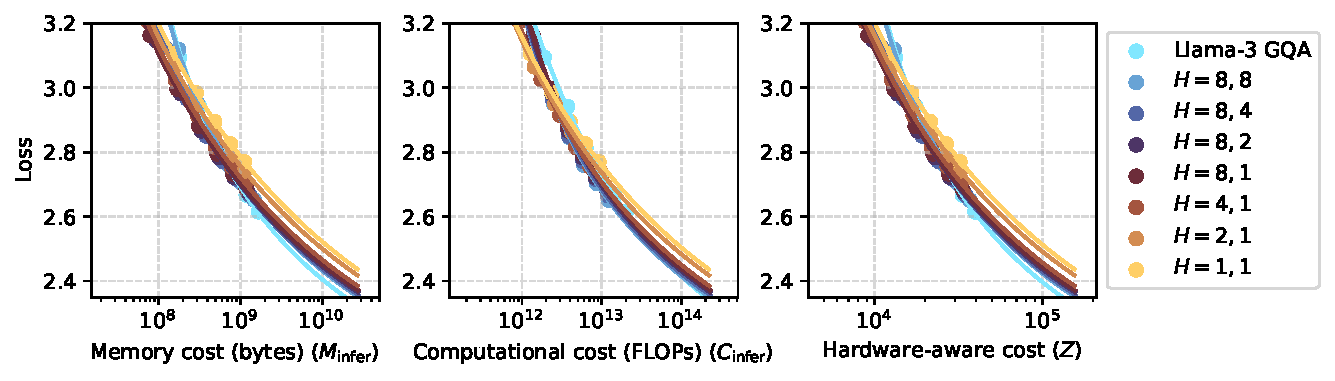
\includegraphics[width=0.95\linewidth]{figures/loss_vs_heads/loss_vs_costs_diff_heads_T-8K.pdf}
    \caption{Loss as a function of memory, computational, and hardware-aware ($Z$ in Section \ref{sec:cost-optimal-gqa-search}) costs during inference with a \textbf{context length of 8K tokens}.}
    \label{fig:loss_vs_H_8k}
\end{figure*}


\begin{figure*}[!t]
    \centering
    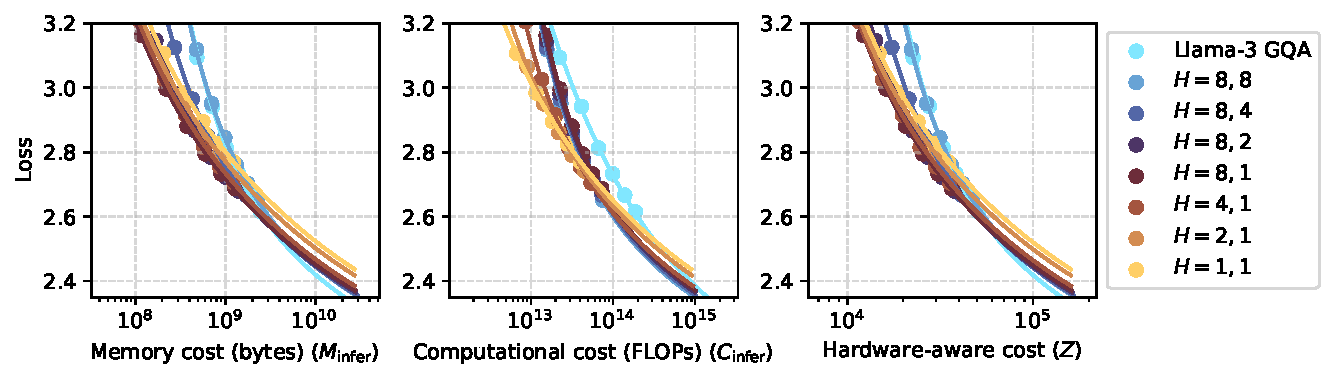
\includegraphics[width=0.95\linewidth]{figures/loss_vs_heads/loss_vs_costs_diff_heads_T-32K.pdf}
    \caption{Loss as a function of memory, computational, and hardware-aware ($Z$ in Section \ref{sec:cost-optimal-gqa-search}) costs during inference with a \textbf{context length of 32K tokens}.}
    \label{fig:loss_vs_H_32k}
\end{figure*}

\begin{figure*}[!t]
    \centering
    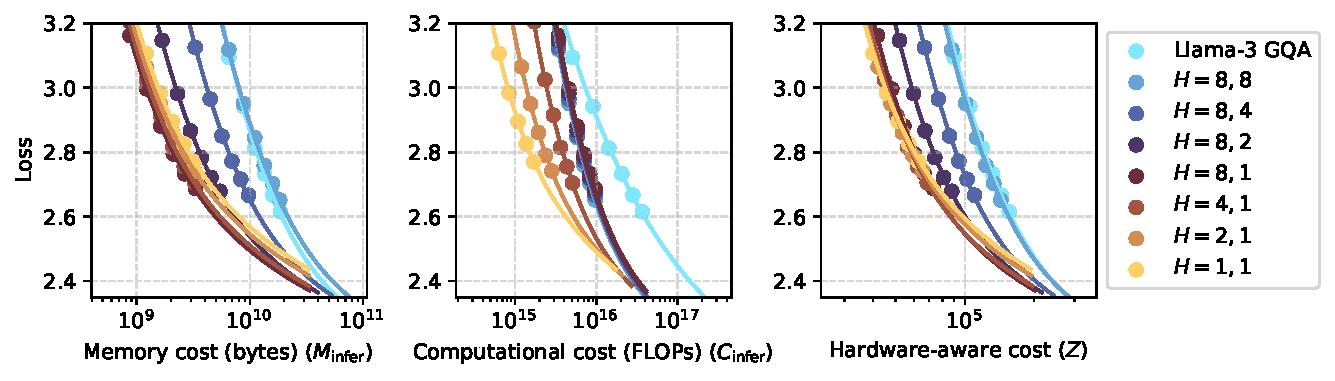
\includegraphics[width=0.98\linewidth]{figures/loss_vs_heads/loss_vs_costs_diff_heads_T-512K.pdf}
    \caption{Loss as a function of memory, computational, and hardware-aware ($Z$ in Section \ref{sec:cost-optimal-gqa-search}) costs during inference with a \textbf{context length of 512K tokens}.}
    \label{fig:loss_vs_H_512k}
    \vspace{-1em}
\end{figure*}


Here, we provide the results for the relationship between loss and inference costs for other context lengths. The results are shown in Figure \ref{fig:loss_vs_H_8k}, \ref{fig:loss_vs_H_32k}, and \ref{fig:loss_vs_H_512k}. We can see that for shorter context lengths, the gain of reducing $n_h$ or $n_{kv}$ is relatively small, but the commonly used GQA ($n_{kv}=8$) configuration is still suboptimal at 32K context length. At 1.2B parameters, GQA uses more FLOPs and memory than $H=8,1$. For longer context lengths such as 512K, we can achieve the same loss with less than 10\% of the original memory usage by using fewer KV heads, but a larger model (increasing $N$).


\subsection{Influence of Query and KV Heads for Different Context Lengths}
\label{sec:appendix-influence-of-H-for-different-T}

Here, we provide the supplementary results for Section~\ref{sec:influence-of-query-and-kv-heads} for other context lengths (8K, 32K, and 512K). Similar to the previous section, a greater context length means that the advantage of using fewer heads is greater. In the following section, we explicitly fit the relationship between loss and $n_h$ and $n_{kv}$ with power-plus-constant functions.


\section{The Scaling Laws of Attention Heads}
\label{sec:appendix-scaling-law-heads}


\begin{figure}[t]
    \centering
    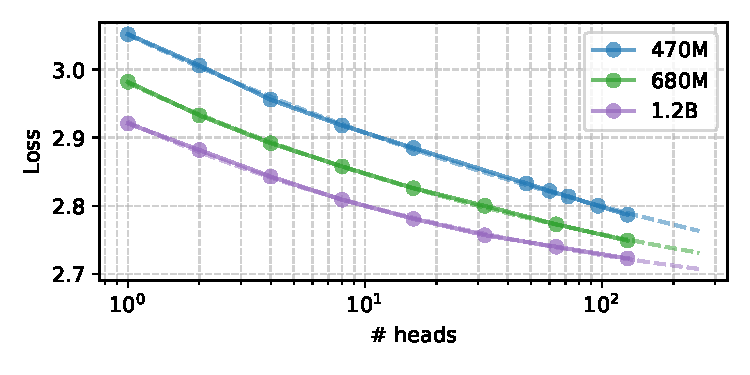
\includegraphics[width=1.0\linewidth]{figures/loss_vs_heads/loss_by_nh_T-1k_diff_N.pdf}
    \caption{The relationship between LM loss and the number of attention heads, fitted with a power-plus-constant function. The training context length is 1K.}
    \label{fig:loss_vs_heads_diff_N}
\end{figure}

\begin{figure}[t]
    \centering
    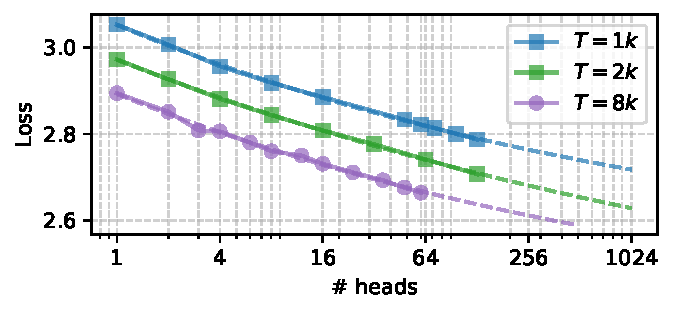
\includegraphics[width=1.0\linewidth]{figures/loss_vs_heads/Loss_vs_nh_diff_T_GPT-470M.pdf}
    \caption{The relationship between LM loss and the number of attention heads, fitted with a power-plus-constant function. The model size is 470M.}
    \label{fig:loss_vs_heads_diff_T}
\end{figure}

In this section, we show that one can predict the loss for a certain head configuration using experiments with a smaller number of heads.
Specifically, we find that---for the first time---the relationship between loss and the number of attention heads closely resembles a power-plus-constant function:
\begin{align*}
    \mathcal L(n_h) = a n_h^b + c
\end{align*}
where $\mathcal L$ is the LM loss, and $a,b,c \in \mathbb R$ are coefficients.
Figure \ref{fig:loss_vs_heads_diff_N} shows that this relationship is observed with different model sizes. The concrete functions for the curves are:
\begin{align*}
    \mathcal L &= 0.579 n_h ^{-0.124} + 2.473 & \text{(470M)} \\
    \mathcal L &= 0.398 n_h ^{-0.177} + 2.583 & \text{(680M)} \\
    \mathcal L &= 0.301 n_h ^{-0.227} + 2.622 & \text{(1.2B)}
\end{align*}
Since the larger model has a greater constant term, this means that these curves will intersect at a certain point (at around $n_h = $ 8K). This is likely incorrect, since the 1.2B model has strictly more parameters than the other models (although at such large values of $n_h$, the relative difference in model size is very small). This means that the fitted curves will break down before $n_h =$ 8K. Fortunately, virtually all LLMs with open weights have fewer than 128 heads, and the fitted curves are very accurate up to 128 heads with $R^2$ values over 0.999. Thus, we conclude that the law is empirically accurate for the vast majority of openly available LLMs.

Similarly, Figure~\ref{fig:loss_vs_heads_diff_T} shows that this trend is consistent across different context lengths. The fitted curves are
\begin{align*}
    \mathcal L &= 1.513 n_h^{-0.039} + 1.53 & (T=1K) \\
    \mathcal L &= 1.436 n_h^{-0.041} + 1.53 & (T=2K) \\
    \mathcal L &= 1.356 n_h^{-0.044} + 1.53 & (T=8K)
\end{align*}
When $n_h$ approaches infinity, the model parameters will be dominated by the attention projection matrices (i.e., QKVO projections). Hence, they converge to the same constant term, which is known as the ``natural entropy of language''. During curve fitting, this constant term is chosen to minimize to fitting error, and we arrive at 1.53. The $R^2$ values of these fits are over 0.999.
% Once again, these curves will likely fall off eventually, but are highly accurate in the typical range. 

From these results, we conclude that this power-plus-constant scaling law between loss and the number of heads is exhibited independently of model size and context length. One important implication of this result is that increasing the number of heads to improve model quality gives diminishing returns. This means that beyond a certain point, the loss reduction brought by further increasing the number of heads is not worth the cost increase.

% Another notable phenomenon is that the gain from using more heads is rather small compared to 

\subsection{Constant Number of KV Heads}

\begin{figure}[t]
    \centering
    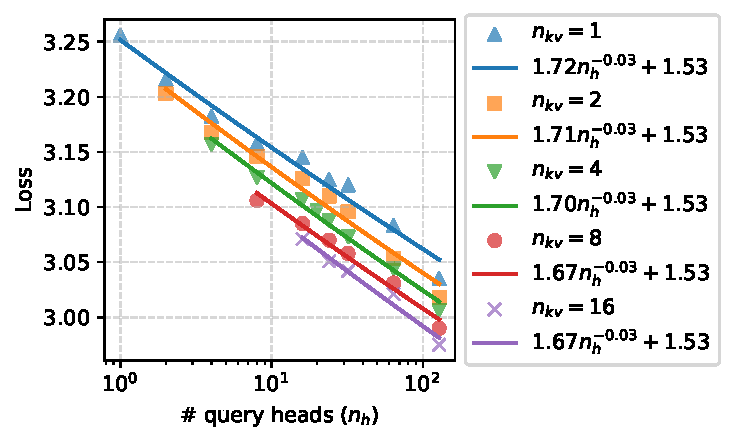
\includegraphics[width=0.98\linewidth]{figures/loss_vs_heads/loss_vs_nh_constant_nkv_150M.pdf}
    \caption{The relationship between loss and $n_h$ when $n_{kv}$ is constant. Model size is 150M.}
    \label{fig:loss_vs_nh_constant_nkv}
\end{figure}


Some LMs (e.g., Llama-3 \citep{llama3}) keep the number of KV heads constant when scaling up the model. Therefore, we also investigate the relationship between LM loss and $n_h$ when $n_{kv}$ is constant. Figure \ref{fig:loss_vs_nh_constant_nkv} shows this relationship with different values of $n_{kv}$ and two model sizes. 
We discover that the relationship is still a power-plus-constant law, but the fitted curves are notably less accurate, with $R^2$ values over 0.97. It is worth noting that the increase in fitting error compared to Section \ref{sec:appendix-scaling-law-heads}) may be attributed to the use of a smaller model (150M vs. 470M).


\section{Experimental Details: Downstream Performance}

This section provides details for Section~\ref{sec:downstream-performance}.

\subsection{Training}
\label{sec:appendix-downtream-training}

The training run for both the Llama-3 GQA and $H=8,1$ (cost-optimal GQA) models are exactly the same. It consists of two phases. The first phase uses the same settings as the scaling experiments in Section~\ref{sec:experimental-settings}. After 20B tokens, we continue training with 128K context length for 1B tokens, using new optimer states. This phase uses a lower maximum LR of 1e-5 for stability and to avoid catastrophic forgetting.


\subsection{Evaluation}
\label{sec:appendix-downstream-eval}

Here, we provide more details regarding the downstream task performance evaluation in Section~\ref{sec:downstream-performance}. We use LM-Evaluation-harness~\citep{eval-harness} for common-sense reasoning, and the needle-in-a-haystack tasks from RULER~\citep{ruler}. For both of these tasks, we evaluate the last four checkpoints of the model, and report the average score of it. This is for reducing the randomness in the results.

\paragraph{Common-Sense Reasoning Tasks} 

We use the popular LM-Evaluation-Harness~\citep{eval-harness} for evaluating common-sense reasoning capabilities. We evaluate on the common-sense reasoning tasks specified by the official implementation, which includes 9 tasks/datasets: ARC-Challenge, ARC-Easy, BoolQ, HellaSwag, Lambada, PIQA, SocialIQA, Wikitext, and Winograd. The scores we report in Table~\ref{tab:downstream-performance} are the average accuracy score (excluding Wikitext, which is evaluated with perplexity). When available, we use the normalized accuracy scores instead of raw accuracy scores.

\paragraph{Retrieval Task}

We report the average accuracy of the synthetic S-NIAH tasks from RULER~\citep{ruler}, which tests the model's ability to retrieve a certain ``needle'' (i.e., some special information) from a large body of irrelevant text.


\subsection{Context Length Extension by Post-Training}

\begin{figure}[!t]
    \centering
    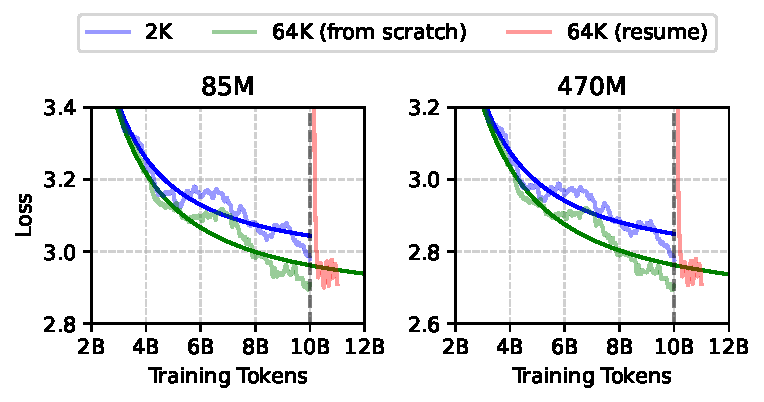
\includegraphics[width=0.98\linewidth]{figures/post-training.pdf}
    \caption{The loss curves of a model with 2K context length adapted to 64K through post-training compared to a model trained with 64K from scratch.}
    \label{fig:post-training}
\end{figure}

LLMs are typically trained on shorter sequences in practice, followed by adaptation to longer contexts using a smaller amount of data tailored to the target context length. To ensure the validity of our conclusions in such training scenarios, we adapted a checkpoint initially trained with a 2K context length to a 64K context length through continual pretraining. This adapted model was then compared to a model trained from scratch with a 64K context length. As illustrated in Figure~\ref{fig:post-training}, the adapted model rapidly converges toward the performance of the model trained from scratch with a 64K context length. This indicates that, with sufficient post-training, the loss of the adapted model approaches that of a model trained entirely from scratch. Consequently, our findings regarding inference costs and the relationship between loss, context length, and head configuration remain applicable to post-training scenarios.


\section{AI Assistance in Research and Writing}

We have used AI for code completion during implementation and grammar-check during paper-writing. We do not explicitly instruct AI to write any part of this paper.
